
\subsection{Skin-Effekt}
Der Widerstand einer stromdurchflossen Leitung hängt neben der Länge und dem Material auch vom Querschnitt des Leiters ab. Dabei rechnet man in der Gleichstromtechnik mit
\begin{equation}
R = \rho \cdot \frac{l}{A}
\end{equation}
wobei $\rho$ der spezifische Widerstand ist. Bei Wechselstrom kommt es jedoch zum sogenannten Skin-Effekt: der Stromfluss im Leiter wird nach außen verdrängt, es fließt also in den äußeren Schichten wesentlich mehr Strom als in den inneren Schichten. Dieser Effekt ist umso stärker, je höher die Frequenz der Spannung ist. Bei den 50 Hz beziehungsweise 60 Hz, die bei den Energienetzen üblich sind, ist der Effekt vergleichsweise schwach.
Erst bei deutlich höheren Frequenzen wird der Effekt so stark, dass der Stromfluss sich praktisch vollständig auf eine dünne Schicht (Haut) beschränkt -- woher der Effekt seinen Namen hat.

Die Stromdichte im Leiter nimmt nach innen hin gemäß
\begin{equation}
j = j_S e^{-\frac{d}{\rho}}
\end{equation}
ab, wobei $j_S$ die Stromdichte am Rand ist und die sogenannte äquivalenten Leitschichtdicke $\rho$ die Tiefe ist, in welcher die Stromdichte auf $1/e$ abgesunken ist. Für Kupfer beträgt der Wert von $\rho$ 9,38 mm (50 Hz) beziehungsweise 8,57 mm (60 Hz). %cite

Der Skineffekt wurde 1873 von J. C. Maxwell vorhergesagt und 1885 von D. E. Hughe erstmals experimentell nachgewiesen\cite{BergmannSchaefer}.

\begin{figure}[tbhn]
\begin{center}
\noindent
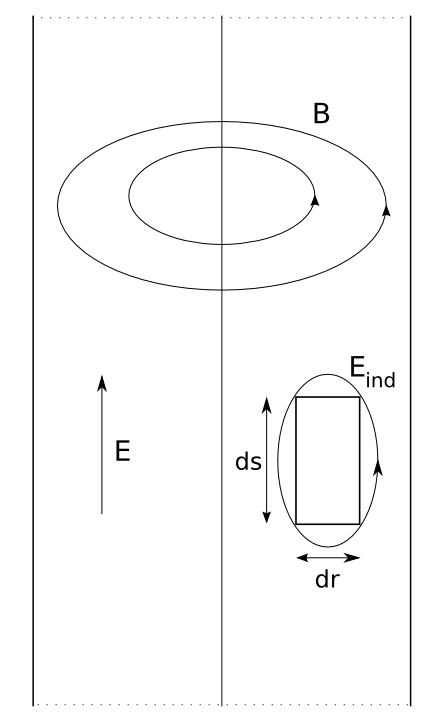
\includegraphics[scale=0.35]{Skineffekt.png}
\end{center}
\caption{Veranschaulichung des Skineffekts: das induzierte elektrische Feld, läuft dem elektrischen Feld der Spannung entgegen.}
\label{pic:skineffekt}
\end{figure}

Zum Verständnis des Effekts betrachten wir ein Flächenelement $ds \cdot dr$ im Drahtinneren (vergleiche Abbildung \ref{pic:skineffekt}).
An dem Draht liegt eine Spannung an, welche also ein elektrisches Feld im Draht erzeugt.
Andererseits fließt durch den Draht ein Strom, durch welchen ein magnetisches Feld aufgebaut wird.
Da es sich um Wechselstrom handelt, ändert das Magnetfeld ständig seine Richtung und Stärke, wodurch ein elektrisches Wirbelfeld induziert wird.
Auf der der Achse zugewandten Seite ist das induzierte elektrische Feld dem äußerem Feld entgegengerichtet, auf der abgewandten Seite gleichgerichtet.
Das resultierende elektrische Feld und somit auch die Stromdichte, muss also von innen nach außen zunehmen.\cite{Gerthsen}

Die genaue Herleitung des Skineffektes ist relativ kompliziert, sie kann in einem Lehrbuch der Elektrodynamik nachgeschlagen werden. % zum beispiel…
Wir wollen hier lediglich eine einfache Herleitung der Eindringtiefe beschreiben. Dabei richten wir uns nach \cite{Gerthsen}, die Herleitung wurde jedoch zur besseren Verständlichkeit ausführlicher als in der Quelle geführt.
Wir starten dabei mit den Maxwellgleichungen, genauer gesagt mit dem Induktionsgesetz von Faraday und dem erweiterten ampèreschen Gesetz:
\begin{align}
\nabla \times \mathbf{E} &= -\frac{\partial \mathbf{B}}{\partial t} \qquad &\mathrm{(Induktionsgesetz\ von\ Faraday)} \\
\nabla \times \mathbf{H} &= \mathbf{j} + \frac{\partial \mathbf{D}}{\partial t} \qquad &\mathrm{(erweitertes\ amp\grave{e}resches\ Gesetz)}
\end{align}
Die elektrische Flussdichte $\mathbf{D}$ hängt mit der elektrischen Feldstärke $\mathbf{E}$ zusammen:
\begin{equation}
\mathbf D = \epsilon_0 \epsilon_r \mathbf{E}
\end{equation}
Da die elektrische Feldstärke von der Spannung abhängt, stellt auch sie eine trigonometrische Funktion von $\omega t$ dar, die Ableitung wird somit zu\footnote{Warum wir hier das $\epsilon_r$ ignorieren können, habe ich leider nicht herausgefunden.}:
\begin{equation}
\mathbf{\dot{D}} = \omega \epsilon_0 \mathbf{E}
\end{equation}
Die Stromdichte $\mathbf{j}$ ergibt sich aus der elektrischen Feldstärke und der elektrischen Leitfähigkeit nach dem ohmschen Gesetz zu $\mathbf{j} = \sigma \mathbf E$. Daraus sehen wir, dass für $\omega \ll \frac{\sigma}{\epsilon} \approx 10^{18} s^{-1}$ $\mathbf{\dot{D}}$ vernachlässigbar klein gegenüber $\mathbf{j}$ ist.

Die magnetische Flussdichte $\mathbf B$ hängt analog mit der magnetischen Feldstärke $\mathbf H$ zusammen:
\begin{equation}
\mathbf B = \mu_0 \mu_r \mathbf H
\end{equation} 
woraus folgt:
\begin{equation}
\mathbf{\dot{B}} = \mu_0 \mu_r \mathbf{\dot{H}}
\end{equation} 
Auf der anderen Seite folgt aus obiger Schreibweise des Ohmschen Gesetzes, dass 
\begin{equation}
\rot \mathbf E = \frac{1}{\sigma} \rot \mathbf{j}
\end{equation}
Damit folgt:
\begin{equation}
\rot \mathbf H = \mathbf{j} \qquad
\rot \mathbf E = \frac{1}{\sigma} \rot \mathbf{j} = \mu_0 \mu_r \mathbf{\dot{H}}
\end{equation}
Daraus wird durch Elimination von $H$
\begin{equation}
\rot\rot \mathbf{j} = \sigma \mu_0 \mu_r \frac{\partial \mathbf{j}}{\partial t}
\end{equation}
Die zeitliche Ableitung entspricht einer Multiplikation mit $\omega$, die zweimalige räumliche Ableitung (rot rot) einer zweimaligen Multiplikation mit der reziproken Schichtdicke, auf der der Strom auf $\frac{1}{e}$ abfällt, und wir erhalten:
\begin{equation}
\frac{1}{d^2} \mathbf{j} \approx \omega \rho \mu_r \mu_0 \mathbf{j}
\end{equation}

